\documentclass[14pt,landscape,color=UCLdarkred,margin=3cm]{uclposter}

\usepackage{amsmath,amssymb}
\usepackage{amsthm}
\usepackage{xcolor}
\usepackage{eso-pic}
\usepackage{authblk}
\usepackage{tikz}
\usepackage{environ}
\usepackage{graphicx}
\usepackage{float}
%\usepackage{physics}

\title{Scalable Quantum Simulation of Molecular Energies}

\author{Shuhao Yang}
\author{James Mills}
\author{Shanice St John}
\affil[1]{Department of LaTeX Studies, UCL}
% \affil[2]{TikZ, UCL}
% \affil[*]{a.example@ucl.ac.uk}

\begin{document}\large

\maketitle

\begin{multicols}{3}

\section*{Introduction}
Quantum computing is a rapidly advancing field predicted to revolutionise many
areas of science and technology. It is predicted to have important real-world applications in encryption and communication systems and in the development of new medicines and materials to name but a few. An important point is that these quantum computers are not considered a replacement to classical computers, they will only be brought to bear on certain types of problems too difficult for classical computers.

Simulating systems in quantum chemistry is one of those problems too difficult for classical computers. If we can efficiently simulate quantum chemistry experiments it would enable a dramatic leap forward in our understanding of fundamental chemistry, and be hugely impactful to a number of fields of endeavour. For example it would significantly reduce the need for cumbersome and expensive trial-and-error techniques in the development of new medicines and materials.


\section*{Highlight boxes}




\begin{highlightbox}[UCLdarkblue!20!white]
	\textbf{Qubit} For representation, we describe information as qubit in quantum mechanics. It is an analogous concept of the classical bit in which classical information is encoded in 0s and 1s.
\end{highlightbox}

\begin{highlightbox}[UCLstone!50!white]
  \textbf{Superposition} A qubit has extraordinary property, which can be in both states of '0' and '1' at the same time, but a classical bit is either `0' or `1'.
\end{highlightbox}

\begin{highlightbox}[UCLmidgreen!20!white]
\textbf{Algorithm} A set of instructions used to solve a problem, especially by a computer. The instructions are created so that it can be understood by the computer. This is then sent to the quantum computer. The computer then follows the instructions using some program or software. The end of the process provides an answer or even many possible answers.
\end{highlightbox}



\columnbreak

\section*{Techniques in Paper}
VQE and PEA are two types of algorithm which is performed by a special type of computer known as the quantum computer.

\subsection*{VQE}

\subsection*{PEA}


\begin{figure}[H]
  \begin{center}
  \begin{minipage}[c]{15em}
    
    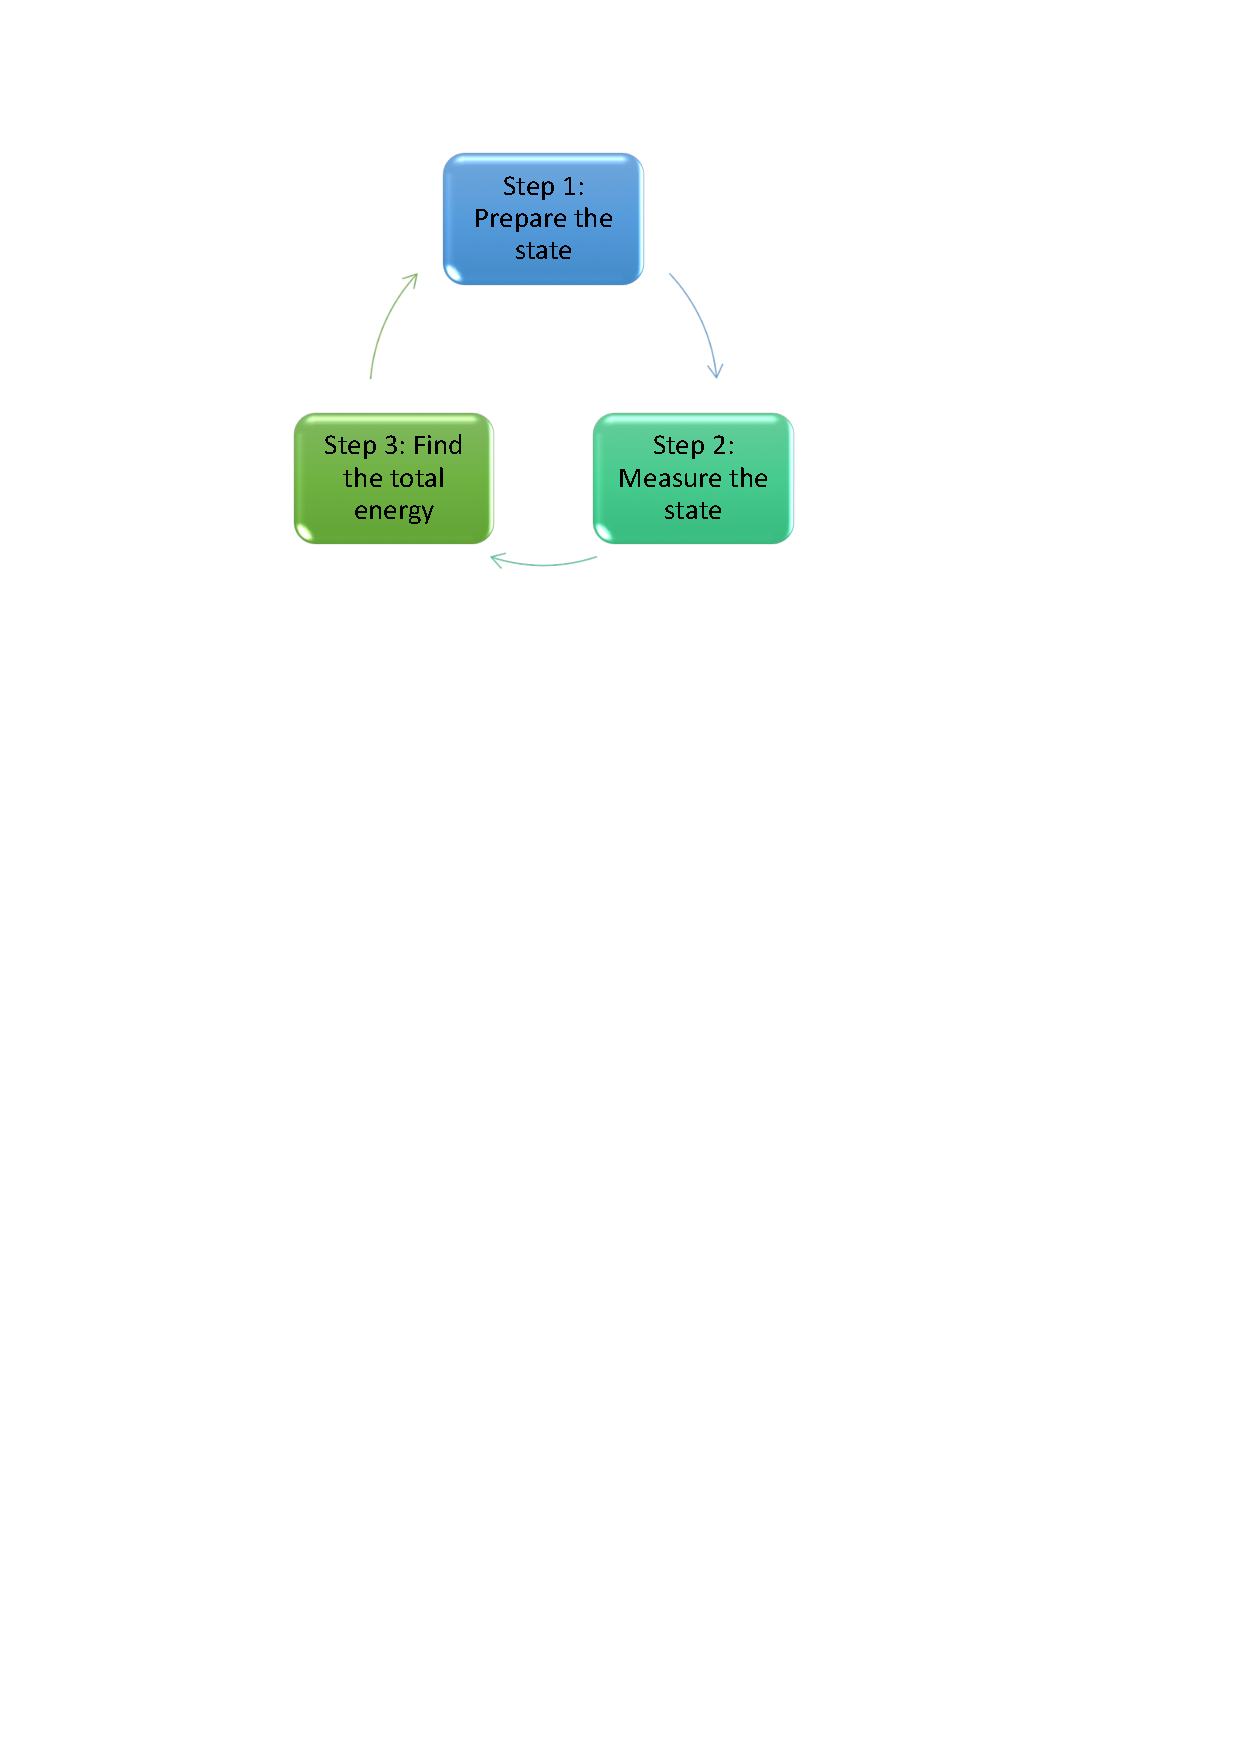
\includegraphics[width=15em]{VQEdiagram.pdf}
    \caption{VQE}
  \end{minipage}
  \qquad
  \begin{minipage}[c]{18em}
    
    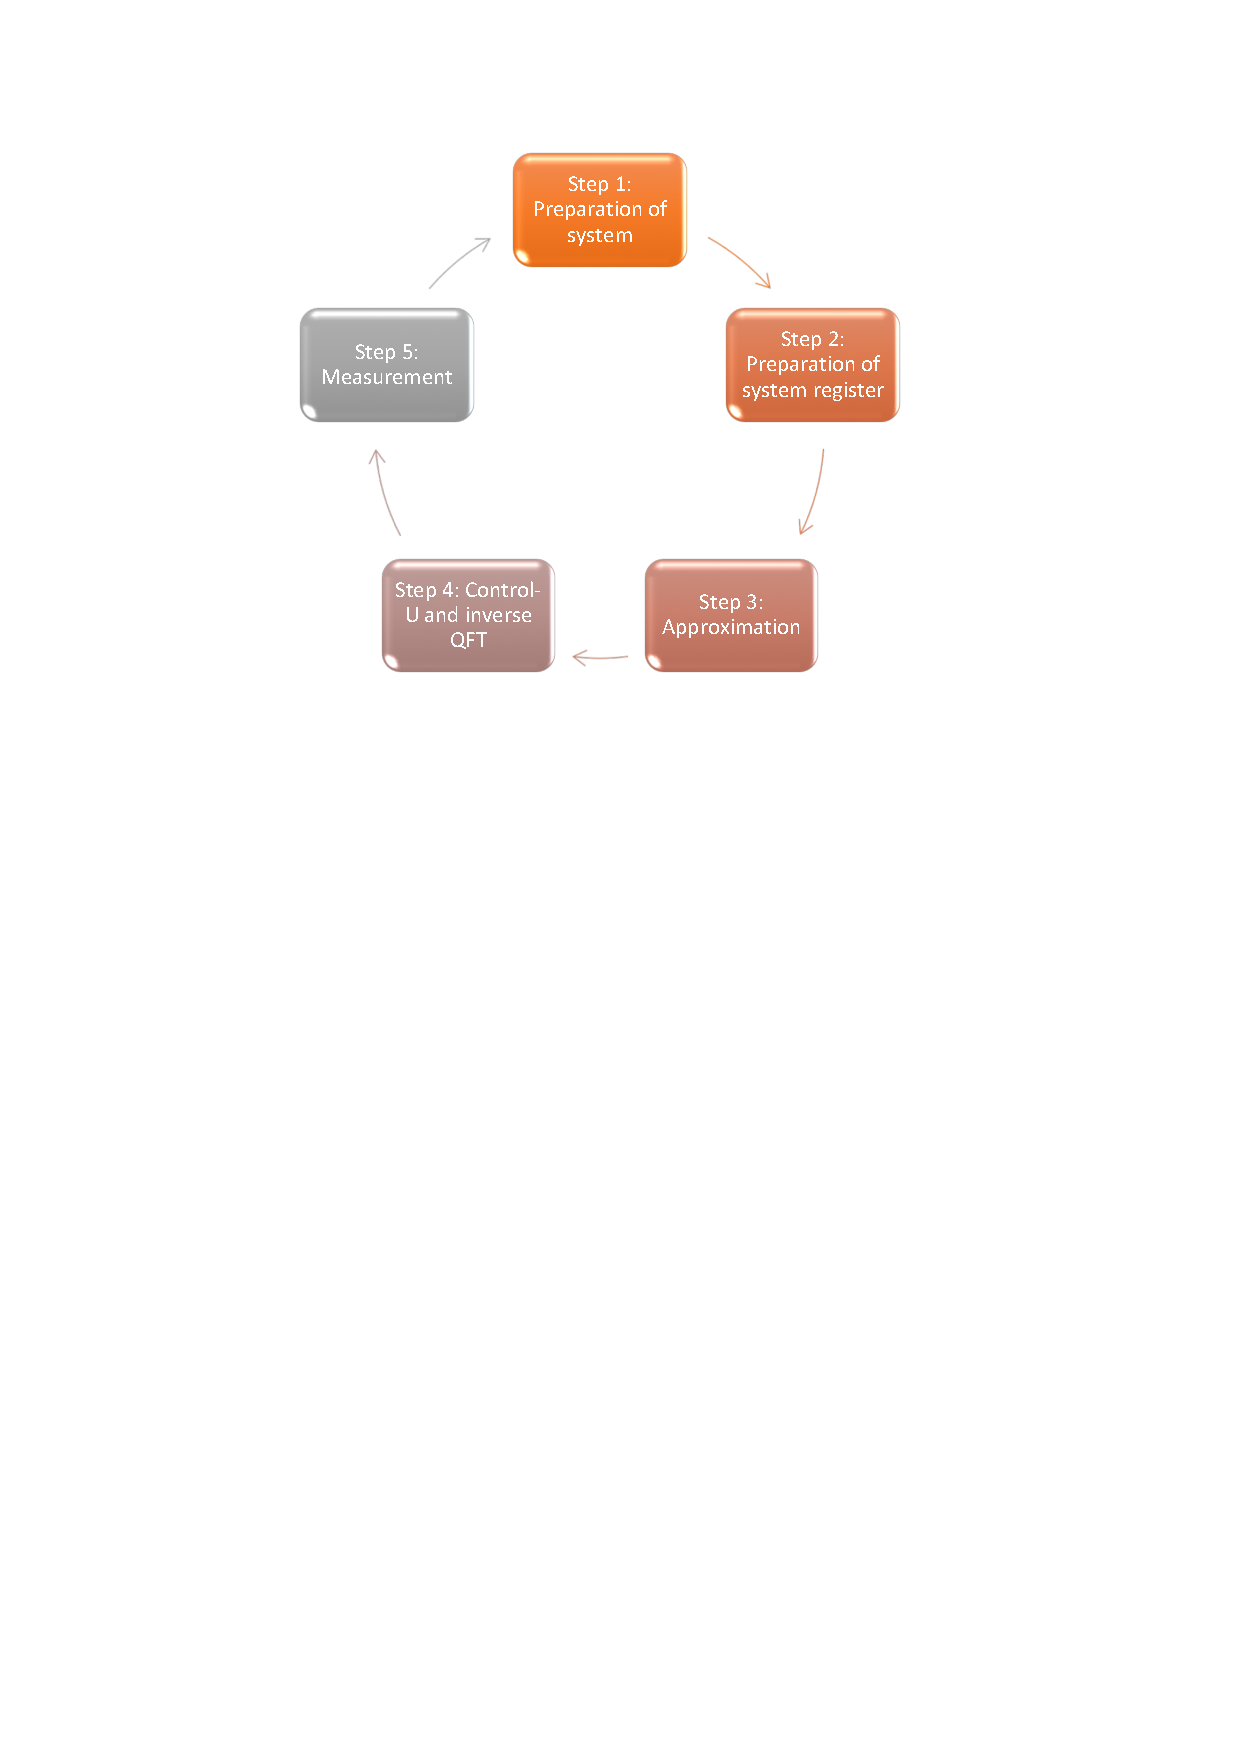
\includegraphics[width=18em]{PEA.pdf}
    \caption{PEA}
  \end{minipage}
  \end{center}

   
\end{figure}



\columnbreak

\section*{Conclusion and Outlook}

\begin{highlightbox}[UCLdarkblue!20!white]
	The colour of a \textbackslash highlightbox can also be changed.
\end{highlightbox}

\begin{figure}[H]
  \begin{center}
  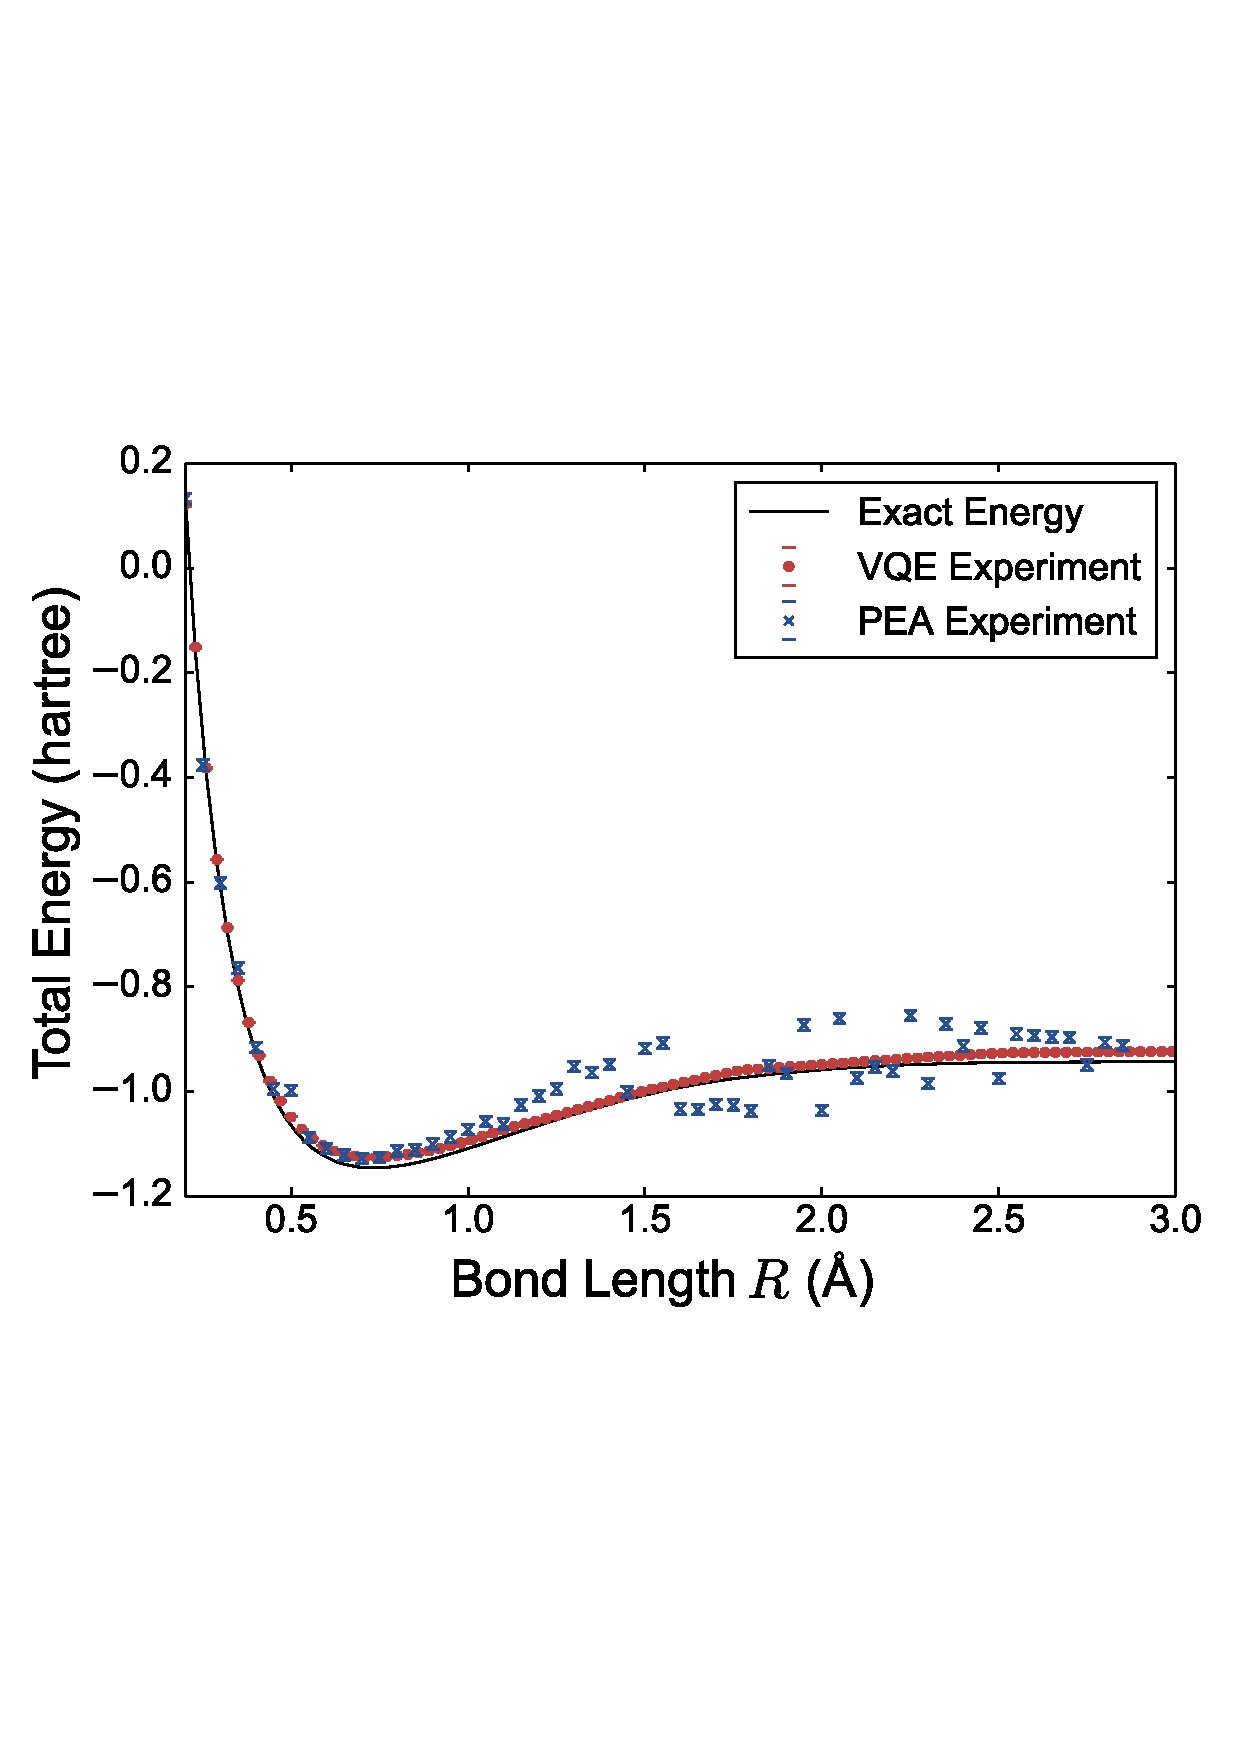
\includegraphics[scale=1.5]{result.pdf}
  \end{center}
    
 

   
\end{figure}




\end{multicols}
	
\end{document}
